\documentclass[12pt]{report}

\usepackage{fouriernc}%la fuente
%\usepackage[sc]{mathpazo} %antigua fuente

\usepackage[utf8]{inputenc}

\usepackage[a4paper,width=150mm,top=25mm,bottom=25mm]{geometry}

\usepackage{subfiles} %esto es para modularizar el overleaf
%para usar este paquete solamente hay que usar el comando
%\subfile{}

\usepackage{graphicx}
\usepackage{framed}
\usepackage[dvipsnames]{xcolor}

\usepackage{xparse}
\usepackage{xstring}

\usepackage{stmaryrd} %para poner el comando \mapsfrom "<---|"

\usepackage{amssymb}

\usepackage{amsmath}
\usepackage{amsthm}

\usepackage{subfig}

\usepackage{mathrsfs} % para tener las fuentes \mathscr que es una letra mayuscula cursiva.

\usepackage{tikz-cd}

\usepackage{tkz-graph}%este paquete es para crear grafos con el ambiente \begin{tikzpicture}

\usepackage{graphicx}

\usepackage{caption}

\usepackage[shortlabels]{enumitem}

\usepackage[sc]{mathpazo}

\usepackage[spanish,activeacute]{babel}

\usepackage{xparse}
\usepackage{xstring}

\usepackage{braket} %para definir \set , \Set y que los conjuntos se vean mas lindos

\usepackage{mathtools}

\usepackage{mathabx}\let\widering\relax %esto es porque hay problemas con el comando \widering que se define en la fuenta fouriernc y en el paquete \usepackage{mathabx}



\usepackage[shortlabels]{enumitem}

\usepackage{hyperref}
\hypersetup{
    colorlinks,
    citecolor=red,
    filecolor=red,
    linkcolor=red,
    urlcolor=red
}

%%%%%%%%%%%%%%%%%%%%%%%%%%%%%%%%%%%%%%%%%%%%%
\theoremstyle{plain}
\newtheorem{theorem}{Teorema}[section]
\newtheorem{lemma}[theorem]{Lema}
\newtheorem{proposition}[theorem]{Proposición}
\newtheorem{proposition/definition}[theorem]{Proposición/Definición}
\newtheorem{corollary}[theorem]{Corolario}
\newtheorem{conjecture}[theorem]{Conjetura}
\newtheorem{afirmacion}[theorem]{Afirmación}
\newtheorem{recuerdo}[theorem]{Recuerdo}

\theoremstyle{definition}
\newtheorem{definition}[theorem]{Definición}
\newtheorem{hypothesis}[theorem]{Hipótesis}
\newtheorem{example}[theorem]{Ejemplo}
\newtheorem{obs}[theorem]{Observación}
\newtheorem{notation}[theorem]{Notación}
\newtheorem{comentario}[theorem]{Comentario}

\newtheorem{exercise}[theorem]{Ejercicio}
%%%%%%%%%%%%%%%%%%%%%%%%%%%%%%%%%%%%%%%%%%%%%




%grupos de matrices
%SL
\newcommand{\SL}[2]{\operatorname{SL}_{#1} ( #2)}
%GL
\newcommand{\GL}[2]{\operatorname{GL}_{#1} ( #2)}

%matriz identidad
\newcommand{\Id}{\operatorname{Id}}



%enteros Z
\newcommand{\integers}{\mathbb{Z}}
%racionales
\newcommand{\rationals}{\mathbb{Q}}
%naturales
\newcommand{\naturals}{\mathbb{N}}
%reales R
\newcommand{\reals}{\mathbb{R}}
%imaginarios
\newcommand{\complex}{\mathbb{C}}
%p-adicos
\newcommand{\padics}{\mathbb{Q}_p}
%enteros p-adicos
\newcommand{\padicintegers}{\mathbb{Z}_p}

%cuerpos finitos
%Fp
\newcommand{\Fp}{\mathbb{F}_p}
%Fq
\newcommand{\Fq}{\mathbb{F}_q}



%valor absoluto p-adico
\newcommand{\abs}[1]{\left \vert #1 \right \vert}
%valor absoluto p-adico
\newcommand{\Abs}[1]{\left \vert \left \vert #1 \right \vert \right \vert}
%valuacion p-adica
\newcommand{\val}[1]{\operatorname{val} (#1)}

%Hom
\newcommand{\Hom}{\operatorname{Hom}}

%imagen y núcleo
\newcommand{\Imagen}{\operatorname{Im}}
\newcommand{\Ker}{\operatorname{Ker}}

%coker
\newcommand{\Coker}{\operatorname{Coker}}

%limite inverso
\newcommand{\liminv}{\varprojlim}


%un poco de typeset para categorias
\newcommand{\catname}[1]{{\operatorfont\textbf{#1}}}


\renewcommand{\hat}[1]{\widehat{#1}}
\renewcommand{\bar}[1]{\overline{#1}}

%declaro un comando nuevo para escribir restricción de funciones
\newcommand\rest[2]{{% we make the whole thing an ordinary symbol
  \left.\kern-\nulldelimiterspace % automatically resize the bar with \right
  #1 % the function
  \vphantom{\big|} % pretend it's a little taller at normal size
  \right|_{#2} % this is the delimiter
  }}


%%%%   COMANDO ALGEBRA CONMUTATIVA   %%%%

%altura de un ideal:
\newcommand{\height}{\textsc{height}}

%Clausura topológica
\newcommand{\closure}[1]{\overline{#1}}

%longitud de un A-modulo. Notacion: \length_A M
\newcommand{\length}{\operatorname{length}}

%Anulador de un $A$-módulo.
\newcommand{\Ann}[1]{\operatorname{Ann} (#1)}

%Cuerpo de fracciones. Notacion $\FracField A$.
\newcommand{\FracField}[1]{\operatorname{Fr} (#1)}


%%%%%%%%%%%%%%%%%%%%%%%%%%%%%%%%%%%%






%%%%   COMANDO TEORÍA DE NÚMEROS  %%%%

%Discriminante
\newcommand{\discriminant}[1]{\mathfrak{d} (#1 )}

%%%%Ideales primos%%%
%escribe una letra en notación mathfrak, para denotar a un ideal o elemento primo.

\newcommand{\primo}[1]{\mathfrak{#1}}
\newcommand{\Primo}[1]{\mathfrak{\MakeUppercase{#1}}}

%anillo de enteros O_K
\renewcommand{\O}{\mathcal{O}}
%anillo de enteros con subindice de cuerpo (input, por ejemplo $K$).
\newcommand{\integralring}[1]{O_{#1}}

%caracteristica de un cuerpo Char k
\newcommand{\Char}[1]{\operatorname{Char} #1}

%traza. Notación \trace = Tr
\newcommand{\trace}{\operatorname{Tr}}

%Traza de extensiones. Notación \Tr L K \alpha = \operatorname{Tr}_{L/K} (\alpha)
\newcommand{\Tr}[1]{\operatorname{Tr}_{L/K} (#1)} %la extension es L/K por default
\newcommand{\tr}[3]{\operatorname{Tr}_{#1/#2} (#3)}

%Norma de extensiones. Notación \Norm L K \alpha = \operatorname{N}_{L/K} (\alpha)
\newcommand{\Norm}[1]{\operatorname{N}_{L/K} (#1)}%la extension es L/K por default
\newcommand{\norm}[3]{\operatorname{N}_{#1/#2} (#3)}


%discriminante de una forma bilineal simetrica. notacion \disc{B} = \operatorname{disc} ( B)
\newcommand{\disc}[1]{\operatorname{disc} (#1)}

%%%%%%%%%%%%%%%%%%%%%%%%%%%%%%%%%%%%

%%%%%%%%%%%%%COMANDO GRAFOS%%%%%%%%%%%%%

%diámetro de un grafo
\newcommand{\diam}[1]{\operatorname{diam} (#1)}

%radio de un grafo
\newcommand{\rad}[1]{\operatorname{rad}(#1)}











%%%%%%%%%%%%%%%%%%%%%%%%%%%%%%%%%%%%



%solución
\newenvironment{solution}{\begin{proof}[Solución]}{\end{proof}}



%%%%%%%%%%%%%%%%%%%%%%%%%%%%%%%

\title{Ejercicio 2 - Entrega 2 - Grafos}
\author{Enzo Giannotta}






\begin{document}

\maketitle

\section{Ejercicio 2 - Entrega 2}

\begin{exercise}
Demuestre o de un contraejemplo: un grafo es bipartito si y solo si ningún par de vértices adyacentes tienen la misma distancia con algún otro vértice.
\end{exercise}
\begin{solution}
\colorlet{shadecolor}{Apricot!12}
\begin{shaded}
\textbf{Sugerencia}: sugiero modificar un poco el enunciado para que no haya ambigüedad. Es decir, si $G$ es un grafo conexo entonces probaremos que, es bipartito si y solo si no existen dos vértices adyacentes distintos a igual distancia de otro vértice (llamemos a esta propiedad $Q$). Para el caso no conexo, simplemente se puede probar que $G$ es bipartito si y solo si cada componente cumple la propiedad $Q$, pues en general si tomamos dos vértices adyacentes $x,y$ luego la distancia a cualquier punto $z$ que no esté en la misma componente que $x,y$ está a distancia $\infty$, es decir, trivialmente $d(x,z) = \infty = d(y,z)$. Recíprocamente, un grafo no conexo que cumple la propiedad $Q$ no es muy divertido, pues si tiene al menos dos vértices, no pueden ser adyacentes (i.e. no tiene aristas) porque de lo contrario habría un tercer vértice en otra componente, en particular a igual distancia $\infty$ de ambos.
\end{shaded}

Supongamos que $G$ es conexo y bipartito. Sea $A\cup B = V(G)$ una partición tal que no hay vértices adyacentes en $A\neq \emptyset$ y $B \neq \emptyset$. Probemos que no existen vértices adyacentes con la misma distancia a otro punto. Sean $x,y$ dos vértices adyacentes, en particular podemos suponer luego de permutar los nombres, que $x \in A$ e $y \in B$. Sea $v \in V(G)$ un vértice, entonces $v \in A$ o $v \in B$, sin pérdida de generalidad supongamos que $v \in A$. Como $G$ es conexo, existen caminos
$$
P_1 = P_{v,x} : x_0=v, x_1, \ldots , x_r=x \quad y \quad P_2 = P_{v,y} : y_0 = v , y_1, \ldots, y_s = y
$$
de longitud mínima, es decir $r = d (x,v)$ y $s = d (y,v)$. Por un lado podemos probar recursivamente que $r$ es par: como $x_0 \in A$ y $x_1$ es adyacente, debe ser que $x_1 \in B$, idénticamente $x_2$ es adyacente a $x_1$, luego $x_2 \in A$, etc, es decir que $x_i \in A$ si y solo si $i$ es par. Esto dice que como $x_r \in A$, $r$ es par. Análogamente, podemos ver que $y_j \in B$ si y solo si $j$ es impar, con lo cual $s$ es impar. Luego, $s \neq r$.

Recíprocamente, supongamos que un grafo conexo $G$ no tiene un par de vértices adyacentes a la misma distancia de otro. Veamos que es bipartito, para eso construyamos una bipartición explícitamente. Sea $v$ un vértice de $G$ fijo, definimos la siguiente partición: consideremos como $A$ al conjunto de los vértices a distancia par de $v$, y $B$ al de los vértices a distancia impar de $v$. Estos conjuntos claramente particionan a $G$, luego nos falta ver que no hay vértices $x,y$ adyacentes, en $A$ o en $B$. En efecto, por el absurdo supongamos que $x,y$ son adyacentes y están en el mismo conjunto (ver la Figura \ref{Figura 1}). Por hipótesis $d(x,v) \neq d(y,v) $, sin pérdida de generalidad supongamos que $d (x,v) < d (y,v)$. Pero también, al estar ambos $x,y$ en $A$ o en $B$, se tiene que $d (x,v)$ y $d ( y,v)$ tienen la misma paridad. Consecuentemenete, $d (x,v) \leq d(y,v) - 2$. Ahora, consideremos un camino $P_{xv}$ entre $x$ y $v$ que realice la distancia entre ambos; tenemos que $y$ no pertenece a $P_{xv}$, ya que de lo contrario se tendría que $d (y,v) \leq d (x,v)$; con lo cual tenemos un camino $yx P_{xv}$ de longitud $d (x,v) +1 < d (y,v)$, entre $y$ y $v$. Imposible.

\begin{center}
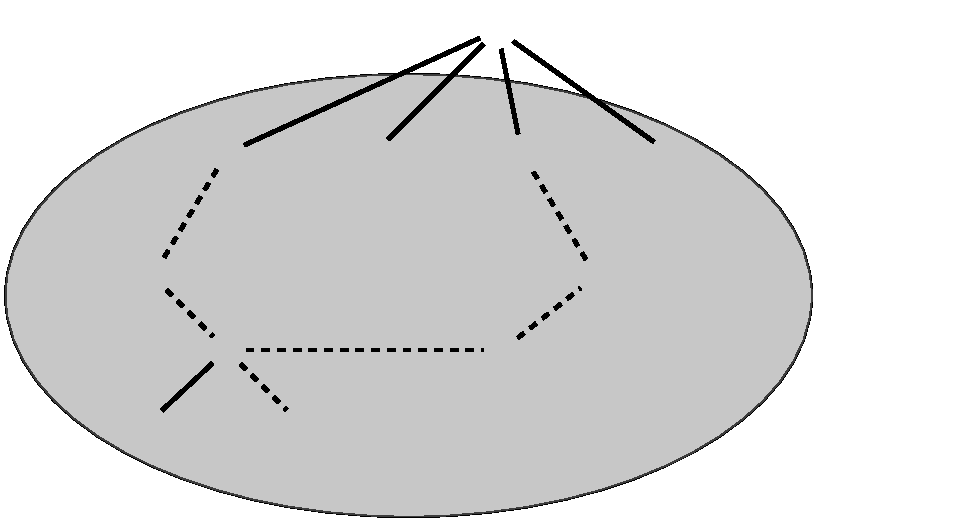
\includegraphics{"./Dibujo 1.pdf"}\label{Figura 1}
\captionof{figure}{Ilustración del absurdo: dos vértices adyacentes dentro del mismo conjunto azul.}
\end{center}

\end{solution}

\end{document}

